\documentclass[conference]{IEEEtran}
\usepackage{amsmath,amssymb,graphicx,booktabs,url,balance}
\usepackage[hidelinks]{hyperref}
\title{BridgeTwin AI: Reproducible Bridge Condition Simulation with Validation-Selected Forecasts and Horizon-Aware Maintenance Planning}
\author{\IEEEauthorblockN{Anonymous Authors}\IEEEauthorblockA{Manuscript prepared for author and supervisor review}}
\begin{document}
\maketitle
\begin{abstract}
A bridge maintenance dashboard can appear convincing even when its forecasts are supported only by synthetic data. This paper presents BridgeTwin AI, a simulation-driven decision-support prototype that makes this distinction explicit. The application connects eight components of a fictional bridge to an interactive three-dimensional view, condition histories, forecasts, scenario comparisons, and budget-constrained interventions. A revised prediction pipeline selects the contribution of machine learning using validation bridges instead of imposing a fixed blend. A revised maintenance objective integrates modeled condition-deficit reduction over a user-selected horizon. Experiments use 15,360 synthetic component-year records from 160 simulated bridges, with disjoint bridge groups for training, validation, calibration, and testing. Validation selects the equation-based predictor without an additional machine-learning contribution. Its one-year test mean absolute error is 0.1021 condition points, compared with 0.1144 for the original fixed blend. In a ten-year scenario with an INR 500,000 budget, horizon-aware selection improves the integrated objective by 20.9\% relative to immediate-benefit selection. These results concern the implemented simulator and configured intervention assumptions. They establish reproducible application behavior, not field accuracy or structural safety.
\end{abstract}
\begin{IEEEkeywords}
bridge maintenance, digital twin prototype, deterioration simulation, model selection, mixed-integer optimization, reproducibility
\end{IEEEkeywords}

\section{Introduction}
Bridge maintenance involves linked decisions: identifying components that need attention, estimating how their condition might change, and allocating a limited budget. A condition score alone does not explain whether repairing a bearing is preferable to protecting several components. A visual model can make the alternatives easier to inspect, but visualization cannot establish the reliability of the underlying forecast.

Digital twin research provides methods for connecting structural observations, predictive models, and maintenance decisions. Torzoni et al. describe a probabilistic framework in which observations update an asset model and inform management actions \cite{torzoni}. Hagen and Andersen discuss damage detection and virtual inspection in a monitored reinforced-concrete bridge \cite{hagen}. These studies also set a useful boundary for a student prototype: an interactive model of a fictional bridge does not provide the same evidence as a monitored physical asset.

BridgeTwin AI therefore uses the term simulation-driven digital twin prototype. Its condition states are proxies produced by explicit assumptions. There is no physical sensor connection, finite-element model, or verified mapping from the displayed score to load-carrying capacity. The application is intended to support exploration of modeling and planning choices.

This work investigates two practical questions. First, should a forecasting system retain a machine-learning contribution when a simpler baseline performs better on validation data? Second, does a repair plan change when benefits are evaluated over the planning horizon rather than immediately after intervention? The contributions are an integrated component-based application, a validation-selected forecasting mixture, and a horizon-aware intervention objective with reproducible comparisons. We do not claim a new regression algorithm or a field-validated deterioration law.

\section{Related Work and Positioning}
A predictive digital twin must relate its state estimates to decisions and uncertainty. The framework in \cite{torzoni} uses a dynamic Bayesian network and reduced-order structural modeling, whereas BridgeTwin AI uses a much simpler, deterministic condition simulator. The monitored case in \cite{hagen} demonstrates a physical-data setting absent from the present experiments. Our contribution is consequently an inspectable software workflow, rather than improved structural diagnosis over these systems.

Random Forests combine randomized tree predictors \cite{breiman}; gradient boosting constructs an additive model through sequential optimization \cite{friedman}. Both are reasonable tabular baselines, but their inclusion does not itself justify better forecasting. In particular, synthetic labels produced from a known equation favor an equation-based baseline. We preserve that baseline in model selection and report the selected result even when it excludes learned predictions.

Residual calibration can help communicate prediction error, but coverage statements depend on the calibration setup and assumptions. Angelopoulos and Bates explain conformal prediction and uncertainty quantification \cite{angelopoulos}. Here, repeated observations within bridges and the use of component residuals for an aggregate chart prevent a direct claim of calibrated bridge-level coverage. The interface labels the displayed bands as illustrative references.

For repair selection, binary decision variables express whether an intervention is chosen. SciPy exposes mixed-integer linear programming through HiGHS \cite{scipy_milp}. We use this established solver and cite the underlying project's recommended algorithm reference \cite{highs}. The study evaluates an application-specific objective; it does not propose a new optimization solver.

\section{System Design}
\subsection{Component State and Data Provenance}
The fictional demonstration asset contains one deck, four piers, one bearing group, and two expansion joints. Each component has a stable identifier shared by the geometric model, API responses, histories, and maintenance actions. A condition score $h_i$ lies between zero and 100. Component weights form an aggregate score
\begin{equation}
H=\frac{\sum_i w_i h_i}{\sum_i w_i}.
\end{equation}
A separate quadratic deficit index emphasizes low-condition components. Neither quantity is a failure probability. A poor component is also shown explicitly so that the average does not become the only information presented to the user.

The React interface uses Three.js for visualization, Zustand for client state, and Recharts for plots. A compatibility renderer supports environments without WebGL. FastAPI provides the application endpoints; SQLite and SQLAlchemy store versioned state, scenario records, dataset metadata, and imported observations. Component selection changes the inspected member without modifying the modeled condition.

The application distinguishes SYNTHETIC, REAL, SIMULATION, and PREDICTION records. REAL is an uploader-supplied label, not verification of authenticity. CSV observations are validated and stored separately from the fictional asset. An import does not silently change the simulation or enter model training. The revised data view reports bridge and component counts, condition ranges, and mean condition, and supports downloading normalized observations.

\subsection{State Consistency and Scenario Isolation}
The server holds the authoritative bridge state. Forecasting and what-if experiments operate on copies. Applying a stress scenario changes the operating inputs at the current simulation date; it does not silently advance the clock to the end of the forecast. Applying repairs changes the current modeled condition and records the intervention.

Every state mutation increments a revision. A maintenance application request must include the revision used in its comparison. A mismatch returns a conflict instead of applying a plan evaluated against old conditions. This matters when another session advances the timeline after a comparison has been generated. Scenario application already follows a similar check. The interface also clears obsolete scenario displays when time advances.

\section{Forecasting Method}
\subsection{Condition Simulator}
Deterioration is integrated in monthly steps. For component $i$, the nominal annual rate is the product of a type-specific base rate and factors for age, loading, environmental exposure, maintenance delay, accumulated loading, material, and protection. Its bounded update is
\begin{equation}
h_{i,t+\Delta t}=\max(0,h_{i,t}-r_i(c_t,e_t)\Delta t).
\end{equation}
Protection decays over time, while age and accumulated loading increase. Intervention assumptions specify an immediate condition gain and a protection value. The coefficients are configured demonstration assumptions. The term equation-based is used deliberately: these relationships are inspired by deterioration reasoning but have not been fitted to structural measurements.

\subsection{Synthetic Data and Grouped Splits}
The supplied generator produces 160 bridges with eight components observed over 12 annual transitions, yielding 15,360 records. Scenarios include normal operation, loading stress, delayed maintenance, ageing, and post-maintenance recovery. A fixed seed of 42 controls generation. Thirteen inputs describe current condition, component type, age, maintenance, material, protection, and operating environment.

Whole bridges are assigned to four disjoint sets: 96 training bridges, 24 validation bridges, 16 calibration bridges, and 24 test bridges. Their row counts are 9,216, 2,304, 1,536, and 2,304, respectively. Group separation prevents the same simulated bridge from appearing in training and testing. It does not create independence between the generator and the equation baseline.

\subsection{Learned Deterioration and Mixture Selection}
Each regressor learns the nonnegative annual condition loss $d_i=\max(0,h_i-y_i)$, rather than directly learning the next score. Predicted loss is subtracted from current condition and clipped to physical score bounds. Random Forest uses 90 trees, maximum depth 16, and a minimum leaf size of three. Gradient Boosting uses 150 estimators, depth three, learning rate 0.08, and Huber loss. Fixed model seeds support repetition.

The model with lower validation MAE is retained. Its bounded prediction $\hat h^{ML}$ is combined with the equation prediction $\hat h^{E}$:
\begin{equation}
\hat h=(1-\alpha)\hat h^{E}+\alpha\hat h^{ML}.
\end{equation}
Unlike the original fixed $\alpha=0.35$, the revised pipeline searches 21 weights from zero to one in increments of 0.05 using validation MAE only. Calibration and test rows are excluded from selection. The zero endpoint allows the system to retain the simpler baseline when learned predictions add no measured benefit. Multi-year forecasts recursively update the component state; this study reports predictive accuracy for the one-year target only.

\begin{figure}[t]
\centering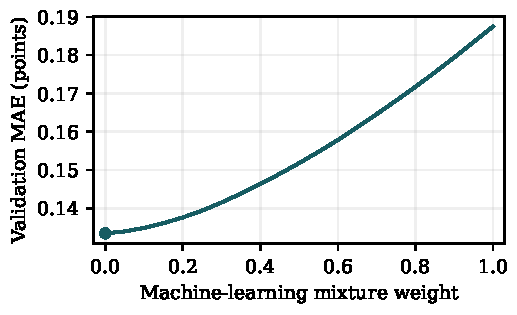
\includegraphics[width=\columnwidth]{blend_selection.pdf}
\caption{Validation error across the fixed mixture-weight grid. The equation-only endpoint is selected without using test rows.}
\label{fig:blend}
\end{figure}

\subsection{Residual Reference Bands}
Absolute one-year residuals on calibration components determine a finite-sample adjusted 90\% residual quantile. Test coverage is measured separately. The chart widens this reference by $\sqrt{t}$ for longer horizons. This is a display heuristic, not a calibrated multi-year interval. Moreover, applying a component residual width around aggregate bridge health does not establish aggregate coverage. The revised interface states these limitations beside the chart.

\section{Horizon-Aware Maintenance Planning}
For each intervention $a$ on component $i$, the application forecasts an untreated and a treated trajectory. The treated trajectory assumes that the repair happens now. Let $q(h)=(100-h)^2/100$. The objective coefficient is
\begin{equation}
b_{ia}(T)=w_i\int_0^T [q(h_i^0(t))-q(h_i^a(t))]_+\,dt,
\end{equation}
computed by trapezoidal integration of annual forecast samples. Its unit is a weighted condition-deficit index-year. Annual samples use the application's rounded forecast scores. This objective captures both immediate recovery and the subsequent effect of protection under the simulator.

Binary variables $x_{ia}$ select interventions:
\begin{align}
\max_x\quad &\sum_{i,a} b_{ia}(T)x_{ia},\\
\text{subject to}\quad &\sum_{i,a} C_{ia}x_{ia}\leq B,\\
&\sum_a x_{ia}\leq 1\quad\forall i,\quad x_{ia}\in\{0,1\}.
\end{align}
The model assumes separable component trajectories, so intervention coefficients can be evaluated before solving. Detailed inspection has no artificial recovery benefit and is excluded from this physical-improvement objective. That exclusion is a limitation: information value is not modeled. The solver also does not enforce mandatory treatment of critical components. Such requirements would need engineering rules and explicit constraints.

The horizon may be selected from one to 20 years. All selected work still occurs at the start; the method does not schedule repeated repairs, crews, closures, or annual budgets. Intervention costs are illustrative INR values, not quotations or life-cycle cost estimates.

\section{Experimental Results}
\subsection{Prediction Comparison}
Table~\ref{tab:prediction} reports one-year results on the untouched synthetic test set. Random Forest has validation MAE 0.1875, compared with 0.2159 for Gradient Boosting, before mixture selection. The mixture search in Fig.~\ref{fig:blend} selects $\alpha=0$, with validation MAE 0.1334. The selected predictor therefore equals the equation baseline in this experiment.
\begin{table}[t]
\caption{One-Year Synthetic Test Results}
\label{tab:prediction}\centering
\begin{tabular}{lrrr}\toprule
Method & MAE & RMSE & $R^2$\\\midrule
Persistence & 2.3783 & 3.2601 & 0.991151\\
Selected Random Forest & 0.1720 & 0.2983 & 0.999926\\
Original 65/35 mixture & 0.1144 & 0.2012 & 0.999966\\
Equation baseline & 0.1021 & 0.1813 & 0.999973\\
Validation-selected mixture & 0.1021 & 0.1813 & 0.999973\\\bottomrule
\end{tabular}
\end{table}
The revised selection reduces MAE by approximately 10.7\% relative to the original mixture. This is a selection improvement within a controlled synthetic experiment, not evidence that structural modeling outperforms ML on real inspection records. The generator uses the same deterioration equations with controlled noise; strong baseline agreement is expected. The high $R^2$ values should be read in that context. The selected residual reference achieves 89.37\% component-row test coverage against a nominal 90\% level. It does not establish bridge-level or multi-year calibration.

\subsection{Budget and Horizon Experiments}
The initial fictional bridge score is 70.03. We evaluate five budgets, INR 0, 500,000, 1,000,000, 2,500,000, and 5,000,000, over horizons of one, five, and ten years. Every plan stays within its budget. The comparison policy maximizes immediate deficit reduction. Both policies are then evaluated on the same integrated objective, avoiding comparison of incompatible units.
\begin{table}[t]
\caption{Selected Planning Comparisons on the Same Objective}
\label{tab:planning}\centering
\begin{tabular}{rrrrr}\toprule
Budget & Years & Immediate plan & Revised plan & Gain\\
(INR) & & objective & objective & (\%)\\\midrule
500,000 & 1 & 32.70 & 32.70 & 0.0\\
500,000 & 10 & 616.72 & 745.81 & 20.9\\
1,000,000 & 5 & 406.41 & 431.27 & 6.1\\
1,000,000 & 10 & 1159.07 & 1316.38 & 13.6\\
2,500,000 & 5 & 653.04 & 653.04 & 0.0\\\bottomrule
\end{tabular}
\end{table}
With INR 500,000, the one-year plan replaces the bearing group for INR 480,000. Over ten years, the revised objective instead selects preventive work on Pier 2, the bearing group, and both joints for the same total cost. The modeled integrated benefit rises from 616.72 to 745.81, a 20.9\% increase. Under these assumptions, distributing protection has a larger accumulated benefit than a single immediate replacement. This is not a recommendation to defer replacement on a real bridge.

With INR 2,500,000 and five years, both policies choose the same six interventions costing INR 2,440,000. The projected aggregate score is 76.25 after repair, compared with 53.05 without new repair. Equal plans in this case show that horizon awareness does not imply a different solution at every budget. The experiment script exports action identifiers, costs, objectives, and forecast endpoints for all 15 combinations.

\subsection{Application Verification}
The revised backend passes 33 automated tests. Checks include grouped split isolation, bounded predictions, feasible budgets, comparison with exhaustive enumeration on a two-component horizon-aware problem, normalized CSV validation, imported-data isolation, download behavior, and stale maintenance rejection. The frontend production build also succeeds. These checks validate software behavior; they do not validate deterioration coefficients, decision efficacy, or bridge safety. No field measurements or independent user study were collected.

\section{Limitations and Future Work}
The principal limitation is the shared synthetic generator. Grouped holdouts reduce bridge overlap, but all groups still arise from the same assumptions. External inspection records, provenance checks, missing-data analysis, and temporal validation are needed before estimating performance on real assets. A useful next experiment would evaluate whether ML learns residual discrepancies after calibrating the equation model on independent observations.

A second limitation is the condition proxy. It does not represent strain, stress, crack geometry, stiffness, or structural capacity. The geometric model is schematic and has no verified BIM or finite-element correspondence. Live sensor assimilation is absent. The prototype therefore demonstrates a decision workflow rather than an operational asset twin.

Third, intervention effects and costs are uncalibrated. The optimizer lacks component dependencies, discounting, uncertainty-aware constraints, repair scheduling, and mandatory engineering intervention rules. Longer horizons amplify assumptions. Multi-year accuracy should be evaluated against independent trajectories, and aggregate uncertainty requires calibration at the bridge level. Repeated seeds and varied deterioration mechanisms would also test sensitivity beyond the single seeded dataset used here.

\section{Conclusion}
BridgeTwin AI connects component visualization, explicit deterioration assumptions, forecasting, and constrained intervention selection in a reproducible application. Validation-selected blending removes an unsupported fixed ML contribution in the supplied synthetic experiment. Horizon-aware planning changes repair priorities for some budget-horizon combinations and matches immediate-benefit planning for others. The value of the prototype is that these outcomes can be inspected and reproduced without presenting simulated condition scores as verified structural measurements. Progress toward real deployment depends on independent data, calibrated models, and engineering constraints.

\balance
\begin{thebibliography}{00}
\bibitem{torzoni} M. Torzoni, M. Tezzele, S. Mariani, A. Manzoni, and K. E. Willcox, ``A digital twin framework for civil engineering structures,'' \emph{Comput. Methods Appl. Mech. Eng.}, vol. 418, Art. no. 116584, 2024, doi: 10.1016/j.cma.2023.116584.
\bibitem{hagen} A. Hagen and T. M. Andersen, ``Asset management, condition monitoring and Digital Twins: damage detection and virtual inspection on a reinforced concrete bridge,'' arXiv:2404.10341, 2024, doi: 10.48550/arXiv.2404.10341.
\bibitem{breiman} L. Breiman, ``Random forests,'' \emph{Machine Learning}, vol. 45, pp. 5--32, 2001, doi: 10.1023/A:1010933404324.
\bibitem{friedman} J. H. Friedman, ``Greedy function approximation: A gradient boosting machine,'' \emph{Ann. Statist.}, vol. 29, no. 5, pp. 1189--1232, 2001, doi: 10.1214/aos/1013203451.
\bibitem{angelopoulos} A. N. Angelopoulos and S. Bates, ``A gentle introduction to conformal prediction and distribution-free uncertainty quantification,'' arXiv:2107.07511, 2021, revised 2022, doi: 10.48550/arXiv.2107.07511.
\bibitem{scipy_milp} SciPy Developers, ``scipy.optimize.milp,'' \emph{SciPy Reference Guide}. Accessed: Nov. 16, 2026. [Online]. Available: \url{https://docs.scipy.org/doc/scipy/reference/generated/scipy.optimize.milp.html}
\bibitem{highs} Q. Huangfu and J. A. J. Hall, ``Parallelizing the dual revised simplex method,'' \emph{Math. Program. Comput.}, vol. 10, no. 1, pp. 119--142, 2018, doi: 10.1007/s12532-017-0130-5.
\end{thebibliography}
\end{document}
